\documentclass[10pt,twocolumn]{article}
\setlength\textwidth{6.875in}
\setlength\textheight{8.875in}
% set both margins to 2.5 pc
\setlength{\oddsidemargin}{-0.1875in}% 1 - (8.5 - 6.875)/2
\setlength{\evensidemargin}{-0.1875in}
\setlength{\marginparwidth}{0pc}
\setlength{\marginparsep}{0pc}%
\setlength{\topmargin}{0in} \setlength{\headheight}{0pt}
\setlength{\headsep}{0pt}
\setlength{\footskip}{37pt}%
\setlength{\columnsep}{0.3125in}
\setlength{\columnwidth}{3.28125in}% (6.875 - 0.3125)/2 = 3.28125in
\setlength{\parindent}{1pc}
\newcommand{\myMargin}{1.00in}
\usepackage[top=\myMargin, left=\myMargin, right=\myMargin, bottom=\myMargin, nohead]{geometry}
\usepackage{epsfig,graphicx}
\usepackage{palatino}
\usepackage{fancybox}
\usepackage[procnames]{listings}

\newenvironment{commentary}
{ \vspace{-0.1in}
  \begin{quotation}
  \noindent
  \small \em
  \rule{\linewidth}{1pt}\\
}
{
  \end{quotation}
}

\title{Chisel Manual}
\author{Jonathan Bachrach, Krste Asanovi\'{c} \\
EECS Department, UC Berkeley\\
{\tt  \{jrb|krste\}@eecs.berkeley.edu}
}
\date{\today}

\newenvironment{example}{\VerbatimEnvironment\begin{footnotesize}\begin{Verbatim}}{\end{Verbatim}\end{footnotesize}}
\newcommand{\kode}[1]{\begin{footnotesize}{\tt #1}\end{footnotesize}}

\def\code#1{{\small\tt #1}}

\def\note#1{\noindent{\bf [Note: #1]}}
%\def\note#1{}

% "define" Scala
\usepackage[T1]{fontenc}  
\usepackage[scaled=0.82]{beramono}  
\usepackage{microtype} 

\sbox0{\small\ttfamily A}
\edef\mybasewidth{\the\wd0 }

\lstdefinelanguage{scala}{
  morekeywords={abstract,case,catch,class,def,%
    do,else,extends,false,final,finally,%
    for,if,implicit,import,match,mixin,%
    new,null,object,override,package,%
    private,protected,requires,return,sealed,%
    super,this,throw,trait,true,try,%
    type,val,var,while,with,yield},
  sensitive=true,
  morecomment=[l]{//},
  morecomment=[n]{/*}{*/},
  morestring=[b]",
  morestring=[b]',
  morestring=[b]"""
}

\usepackage{color}
\definecolor{dkgreen}{rgb}{0,0.6,0}
\definecolor{gray}{rgb}{0.5,0.5,0.5}
\definecolor{mauve}{rgb}{0.58,0,0.82}

% Default settings for code listings
\lstset{frame=tb,
  language=scala,
  aboveskip=3mm,
  belowskip=3mm,
  showstringspaces=false,
  columns=fixed, % basewidth=\mybasewidth,
  basicstyle={\small\ttfamily},
  numbers=none,
  numberstyle=\footnotesize\color{gray},
  % identifierstyle=\color{red},
  keywordstyle=\color{blue},
  commentstyle=\color{dkgreen},
  stringstyle=\color{mauve},
  frame=single,
  breaklines=true,
  breakatwhitespace=true,
  procnamekeys={def, val, var, class, trait, object, extends},
  procnamestyle=\ttfamily\color{red},
  tabsize=2
}

\lstnewenvironment{scala}
{\lstset{language=scala}}
{}
\lstnewenvironment{cpp}
{\lstset{language=C++}}
{}
\lstnewenvironment{bash}
{\lstset{language=bash}}
{}
\lstnewenvironment{verilog}
{\lstset{language=verilog}}
{}



\lstset{frame=}

\begin{document}
\maketitle{}

% TODO: default
% TODO: enum yields Bits
% TODO: why hardware construction languages



\section{Introduction}

This document is a manual for {\em Chisel} (Constructing Hardware In a
Scala Embedded Language).  Chisel is a hardware construction language
embedded in the high-level programming language Scala.  A separate
Chisel tutorial document provides a gentle introduction to using
Chisel, and should be read first.  This manual provides a
comprehensive overview and specification of the Chisel language, which
is really only a set of special class definitions, predefined objects,
and usage conventions within Scala.  When you write a Chisel program
you are actually writing a Scala program.  In this manual, we presume
that you already understand the basics of Scala.  If you are
unfamiliar with Scala, we recommend you consult one of the excellent
Scala books (\cite{programming-scala}, \cite{programming-in-scala}).

\section{Nodes}

Any hardware design in Chisel is ultimately represented by a graph of
node objects.  User code in Chisel generate this graph of nodes, which
is then passed to the Chisel backends to be translated into Verilog or
C++ code.  Nodes are defined as follows:

\begin{scala}
class Node {
  // name assigned by user or from introspection
  var name: String = ""
  // incoming graph edges
  def inputs: ArrayBuffer[Node]
  // outgoing graph edges
  def consumers: ArrayBuffer[Node]
  // node specific width inference
  def inferWidth: Int
  // get width immediately inferrable
  def getWidth: Int
  // get first raw node
  def getRawNode: Node
  // convert to raw bits 
  def toBits: Bits
  // convert to raw bits 
  def fromBits(x: Bits): this.type
  // return lit value if inferrable else null
  def litOf: Lit
}
\end{scala}


The uppermost levels of the node class hierarchy are shown in
Figure~\ref{fig:node-hierarchy}.  The basic categories are:

\begin{description}
\item[Lit] -- constants or literals,
\item[Op] -- logical or arithmetic operations,
\item[Updateable] -- conditionally updated nodes,
\item[Data] -- typed wires or ports,
\item[Reg] -- positive-edge-triggered registers, and
\item[Mem] -- memories.
\end{description}

\begin{figure}[h]
\centering
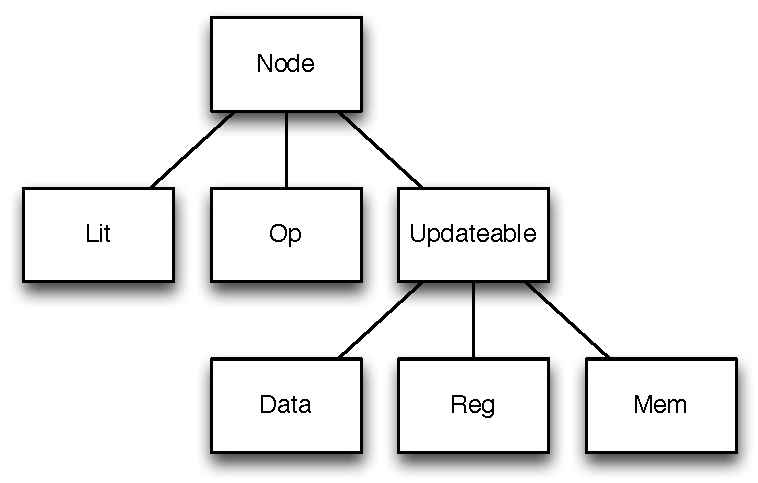
\includegraphics[width=3in]{figs/node-hierarchy.pdf}
\caption{Node hierarchy.}
\label{fig:node-hierarchy}
\end{figure}

\section{Lits}

Raw literals are represented as \code{Lit} nodes defined as follows:

\begin{scala}
class Lit extends Node {
  // original value
  val inputVal: BigInt
}
\end{scala}

\noindent
Raw literals contain a collection of bits.  
Users do not create raw literals directly, but instead use type
constructors defined in Section~\ref{sec:types}.

% Constant or literal values are expressed using Scala integers or strings passed to constructors for the types:

% TODO: isLit and litOf

\section{Ops}

Raw operations are represented as \code{Op} nodes defined as follows:

\begin{scala}
class Op extends Node {
  // op name used during emission
  val op: String
}
\end{scala}

\noindent
Ops compute a combinational function of their inputs.

\section{Types}
\label{sec:types}

A Chisel graph contains {\em raw} and {\em type} nodes.  Type nodes
are interspersed between raw nodes and allow Chisel code to check and
respond to Chisel types.  The Chisel type system is maintained
separately from the underlying Scala type system.  Chisel type nodes
are erased before emission to C++ and Verilog.
Figure~\ref{fig:type-hierarchy} shows the built-in Chisel type
hierarchy, with \code{Data} as the topmost node.

\begin{figure}[h]
\centering
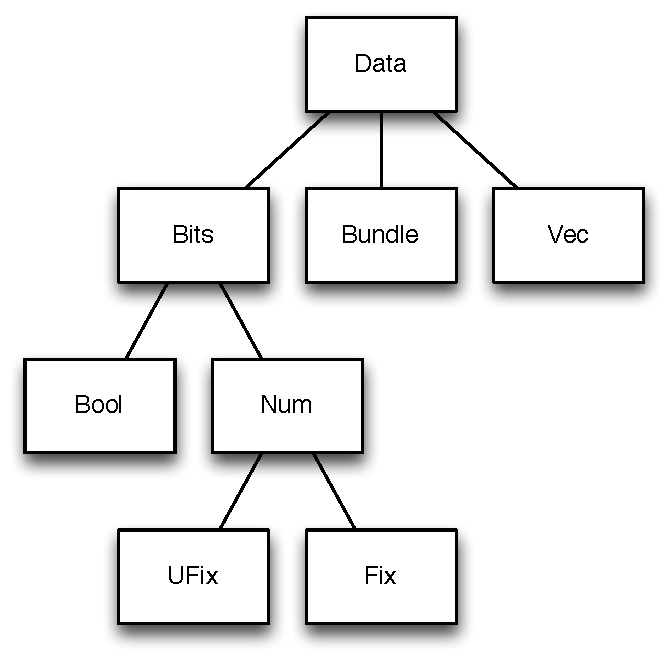
\includegraphics[height=2.5in]{figs/type-hierarchy.pdf}
\caption{Chisel type hierarchy.}
\label{fig:type-hierarchy}
\end{figure}

\noindent
Built-in scalar types include \code{Bits}, \code{Bool}, \code{Fix},
and \code{UFix} and built-in aggregate types \code{Bundle} and
\code{Vec} allow the user to expand the set of Chisel datatypes with
collections of other types.

\code{Data} itself is a node:
\begin{scala}
abstract class Data extends Node {
  override def clone(): this.type =
    this.getClass.newInstance.
      asInstanceOf[this.type]
  // simple conversions
  def toFix: Fix
  def toUFix: UFix
  def toBool: Bool
  def toBits: Bits
  // data leaves if aggregate
  def leaves: Array[(String, Data)]
  // port direction if leaf
  def dir: PortDir
  // change dir to OUTPUT
  def asOutput: this.type
  // change dir to INPUT
  def asInput: this.type
  // change polarity of dir
  def flip: this.type
  // assign to input
  def :=[T <: Data](t: T)
  // bulk assign to input
  def <>(t: Data)
}
\end{scala}
\noindent
The Data class has methods for converting between types and for
delegating port methods to its single input.  We will discuss ports in
Section~\ref{sec:ports}.  Finally, users can override the \code{clone}
method in their own type nodes (e.g., bundles) in order to reflect
construction parameters that are necessary for cloning.

Data nodes can be used for four purposes:

\begin{itemize}
\item {\bf types} -- \kode{UFix(width = 8)} -- record intermediate types in the graph
  specifying at minimum bitwidth (described in this section), 
\item {\bf wires} -- \kode{UFix(width = 8)} -- serve as forward declarations of data allowing future
  conditional updates (described in Section~\ref{sec:wires}), 
\item {\bf ports} -- \kode{UFix(width = 8, dir = OUTPUT)} -- are
  specialized wires defining component interfaces, and
  additionally specify direction (described in
  Section~\ref{sec:ports}), and
\item{\bf literals} -- \kode{UFix(1)} or \kode{UFix(1, 8)} -- can be constructed using type object
constructors specifying their value and optional width.
\end{itemize}

\subsection{Bits}

In Chisel, a raw collection of bits is represented by the \code{Bits}
type defined as follows:

\begin{scala}
object Bits {
  def apply(width: Int = -1, 
            dir: PortDir = null): Bits
  // create literal from BigInt or Int
  def apply(value: BigInt, width: Int = -1): Bits
  // create literal from String using 
  // base_char digit+ string format
  def apply(value: String, width: Int = -1): Bits
}

class Bits extends Data with Updateable {
  // bitwise-not
  def unary_~(): Bits
  // bitwise-and
  def &  (b: Bits): Bits
  // bitwise-or
  def |  (b: Bits): Bits
  // bitwise-xor
  def ^  (b: Bits): Bits
  // and-reduction
  def andR(): Bool
  // or-reduction
  def orR():  Bool
  // xor-reduction
  def xorR():  Bool
  // logical NOT
  def unary_!(): Bool
  // logical AND
  def && (b: Bool): Bool
  // logical OR
  def || (b: Bool): Bool
  // equality
  def ===(b: Bits): Bool
  // inequality
  def != (b: Bits): Bool
  // logical left shift
  def << (b: UFix): Bits
  // logical right shift
  def >> (b: UFix): Bits
  // concatenate
  def ## (b: Bits): Bits
  // extract single bit, LSB is 0
  def apply(x: Int): Bits
  // extract bit field from end to start bit pos
  def apply(hi: Int, lo: Int): Bits
}

def Cat[T <: Data](elt: T, elts: T*): Bits
\end{scala}

\noindent
Bits has methods for simple bit operations.  
Note that \code{\#\#} is binary
concatenation, while \code{Cat} is an n-ary concatentation.
To avoid colliding with Scala's builtin \code{==},
Chisel's bitwise comparison is named \code{===}.

A field of width \code{n} can be created from a single bit using \code{Fill}:
\begin{scala}
def Fill(n: Int, field: Bits): Bits
\end{scala}

\noindent
and two inputs can be selected using \code{Mux}:

\begin{scala}
def Mux[T <: Data](sel: Bits, cons: T, alt: T): T
\end{scala}

\noindent

Constant or literal values are expressed using Scala integers or
strings passed to constructors for the types:
\begin{scala}
Bits(1)       // decimal 1-bit lit from Scala Int.
Bits("ha")    // hex 4-bit lit from string.
Bits("o12")   // octal 4-bit lit from string.
Bits("b1010") // binary 4-bit lit from string.
\end{scala}

\noindent
producing a \code{Lit} as shown in the
leftmost subfigure of Figure~\ref{fig:bits-expressions}.

Operations return an actual operator node with a type node combining
the input type nodes.  See Figure~\ref{fig:bits-expressions} for
successively more complicated examples.

\begin{figure*}
\begin{center}
\begin{tabular}{ccc}
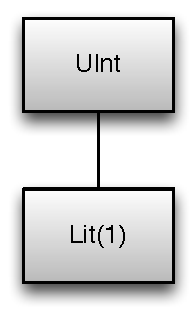
\includegraphics[height=0.94in]{figs/bits-1.pdf} &
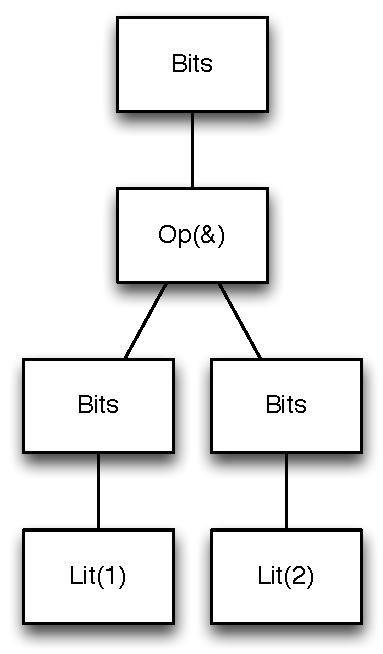
\includegraphics[height=1.96in]{figs/bits-and.pdf} &
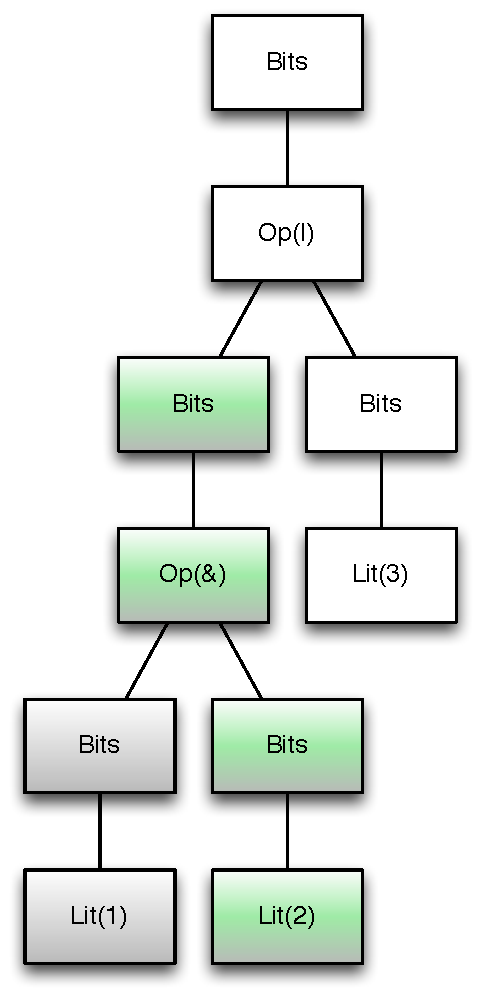
\includegraphics[height=3.0in]{figs/bits-or-and.pdf} \\
\kode{Bits(1)} & \kode{Bits(1) \& Bits(2)} &
\kode{(Bits(1) \& Bits(2)) | Bits(3)} \\
\end{tabular}
\end{center}
\caption{Chisel Op/Lit graphs constructed with algebraic expressions
  showing the insertion of type nodes.}
\label{fig:bits-expressions}
\end{figure*}

\noindent
The \code{getRawNode} operator skips type nodes returning the first
found raw node.

\subsection{Bools}

Boolean values are represented as \code{Bool}s:

\begin{scala}
object Bool {
  def apply(dir: PortDir = null): Bool
  // create literal
  def apply(value: Boolean): Bool
}

class Bool extends Bits
\end{scala}

\noindent
\code{Bool} is equivalent to \code{Bits(width = 1)}.

\subsection{Nums}

\code{Num} is a type node which defines arithmetic operations:

\begin{scala}
class Num extends Bits {
  // Negation
  def unary_-(): Bits
  // Addition
  def +(b: Num): Num
  // Subtraction
  def -(b: Num): Num
  // Multiplication
  def *(b: Num): Num
  // Modulus
  def %(b: Num): Num
  // Division
  def /(b: Num): Num
  // Greater than
  def >(b: Num): Bool
  // Less than
  def <(b: Num): Bool
  // Less than or equal
  def <=(b: Num): Bool
  // Greater than or equal
  def >=(b: Num): Bool
}
\end{scala}

Signed and unsigned integers
are considered subsets of fixed-point numbers and are represented by
types \code{Fix} and \code{UFix} respectively:

\begin{scala}
object Fix {
  def apply (width: Int = -1, 
             dir: PortDir = null): Fix
  // create literal
  def apply (value: BigInt, width: Int = -1): Fix
  def apply (value: String, width: Int = -1): Fix
}

class Fix extends Num 

object UFix {
  def apply(width: Int = -1, 
            dir: PortDir = null): UFix
  // create literal
  def apply(value: BigInt, width: Int = -1): UFix
  def apply(value: String, width: Int = -1): UFix
}

class UFix extends Num {
  // arithmetic right shift
  override def >> (b: UFix): Fix
}
\end{scala}

\noindent
Signed fixed-point
numbers, including integers, are represented using two's-complement
format.  

\subsection{Bundles}

Bundles group together several named fields of potentially different
types into a coherent unit, much like a \code{struct} in C:

\begin{scala}
class Bundle extends Data {
  // shallow named bundle elements
  def elements: ArrayBuffer[(String, Data)]
}
\end{scala}

\noindent
A user can get the name and type corresponding to each element in a
Bundle with the \code{elements} method and recursively using the
\code{leaves} method. 
Users can define their own by subclassing \code{Bundle} as follows:

\begin{scala}
class MyFloat extends Bundle {
  val sign        = Bool()
  val exponent    = Bits(width = 8)
  val significand = Bits(width = 23)
}
\end{scala}

\noindent
and access their elements using Scala field access:

\begin{scala}
val x  = new MyFloat()
val xs = x.sign
\end{scala}

Bundles elements get their emitted names from their bundle field names
which are obtained using Scala introspection.

\subsection{Vecs}

Vecs create an indexable vector of elements: 

\begin{scala}
object Vec {
  def apply[T <: Data](n: Int)(type: => T): Vec[T]
  def apply[T <: Data](elts: Seq[T])(type: => T): Vec[T]
  def apply[T <: Data](elts: T*)(type: => T): Vec[T]
}

class Vec[T <: Data](n: Int, val type: () => T) 
    extends Data {
  def apply(idx: UFix): T
  def apply(idx: Int): T
}
\end{scala}

\noindent
with \code{n} elements of type defined with the \code{gen} thunk.
Users can access elements statically with an \code{Int} index or
dynamically using a \code{UFix} index, 
where dynamic access creates a virtual type node (representing a read
``port'') that records the read using the given address.  In either case,
users can wire to the result of a read as follows:

\begin{scala}
v(a) := d
\end{scala}

% TODO: conditionally assigning to elements

\subsection{Bit Width Inference}

Users are required to set bitwidths of ports and registers, but otherwise,
bit widths on nodes are automatically inferred unless set manually by
the user (using \code{Extract} or \code{Cat}).
The bit-width inference engine starts from the graph's input ports and 
calculates node output bit widths from their respective input bit widths according to the following set of rules:\\[-2mm]

{\small
\begin{tabular}{ll}
{\bf operation} & {\bf bit width} \\ 
\verb|z = x + y| & \verb+wz = max(wx, wy)+ \\
\verb+z = x - y+ & \verb+wz = max(wx, wy)+\\
\verb+z = x & y+ & \verb+wz = max(wx, wy)+ \\
\verb+z = Mux(c, x, y)+ & \verb+wz = max(wx, wy)+ \\
\verb+z = w * y+ & \verb!wz = wx + wy! \\
\verb+z = x << n+ & \verb!wz = wx + maxNum(n)! \\
\verb+z = x >> n+ & \verb+wz = wx - minNum(n)+ \\
\verb+z = Cat(x, y)+ & \verb!wz = wx + wy! \\
\verb+z = Fill(n, x)+ & \verb+wz = wx * maxNum(n)+ \\
% \verb+z = x < y+ & \verb+<= > >= && || != ===+ & \verb+wz = 1+ \\
\end{tabular}
}
\\[1mm]
\noindent  
where for instance $wz$ is the bit width of wire $z$, and the \verb+&+
rule applies to all bitwise logical operations.

The bit-width inference process continues until no bit width changes.
Except for right shifts by known constant amounts, the bit-width
inference rules specify output bit widths that are never smaller than
the input bit widths, and thus, output bit widths either grow or stay
the same.  Furthermore, the width of a register must be specified by
the user either explicitly or from the bitwidth of the reset value.
From these two requirements, we can show that the bit-width inference
process will converge to a fixpoint.

\section{Updateables}

\label{sec:wires}

When describing the operation of wire and state
nodes, it is often useful to instead specify when updates to the
wires and state will occur and to specify these updates spread across
several separate statements.  
For example, Data nodes can be used immediately, but their input set later.
\code{Updateable} represents a conditionally updateable node which
collects accesses and code generates a mux input for the node:

\begin{scala}
abstract class Updateable extends Node {
  // conditional reads
  def reads: Queue[(Bool, UFix)]
  // conditional writes
  def writes: Queue[(Bool, UFix, Node)]
  // gen mux integrating all conditional writes
  def genMuxes(default: Node)
  override def := (x: Node): this.type
}
\end{scala}

Chisel provides conditional update rules
in the form of the \code{when} construct to support this style of
sequential logic description:
 
\begin{scala}
object when {
  def apply(cond: Bool)(block: => Unit): when
}

class when (prevCond: Bool) {
  def elsewhen (cond: Bool)(block: => Unit): when
  def otherwise (block: => Unit): Unit
}
\end{scala}

\noindent
\code{when} manipulates a global condition stack with dynamic scope.
Therefore, \code{when} creates a new condition that is in force across
function calls.  For example:

\begin{scala}
def updateWhen (c: Bool, d: Data) =
  when (c) { r := d }
when (a) { 
  updateWhen(b, x)
}
\end{scala}

\noindent
is the same as:

\begin{scala}
when (a) { 
  when (b) { r := x } 
}
\end{scala}

% TODO: talk about conds

Chisel provides some syntactic sugar for other common forms of
conditional updates:

\begin{scala}
def unless(c: Bool)(block: => Unit) = 
  when (!c) { block )
\end{scala}

\noindent 
and

\begin{scala}
def otherwise(block: => Unit) = 
  when (Bool(true)) { block }
\end{scala}

We introduce the \code{switch} statement for conditional updates
involving a series of comparisons against a common key:

\begin{scala}
def switch(c: Bits)(block: => Unit): Unit

def is(v: Bits)(block: => Unit)
\end{scala}

\section{Forward Declarations}

Purely combinational circuits cannot have cycles between nodes, and
Chisel will report an error if such a cycle is detected.  Because they
do not have cycles, combinational circuits can always be constructed
in a feed-forward manner, by adding new nodes whose inputs are derived
from nodes that have already been defined.  Sequential circuits
naturally have feedback between nodes, and so it is sometimes
necessary to reference an output wire before the producing node has
been defined.  Because Scala evaluates program statements
sequentially, we have allow data nodes to serve as a wire providing
a declaration of a node that can be used immediately, but whose
input will be set later.  
For example, in a simple CPU, we need to define the \verb!pcPlus4!
and \verb!brTarget! wires so they can be referenced before defined:
\begin{scala}
val pcPlus4  = UFix()
val brTarget = UFix()
val pcNext   = Mux(pcSel, brTarget, pcPlus4)
val pcReg    = Reg(pcNext)
pcPlus4     := pcReg + UFix(4)
...
brTarget    := addOut
\end{scala}

\noindent
The wiring operator
\verb!:=! is used to wire up
the connection after \verb!pcReg! and \verb!addOut! are defined.
After all assignments are made and the circuit is being elaborated, 
it is an error if a forward declaration is unassigned.

\section{Regs}

The simplest form of state element supported by Chisel is a
positive-edge-triggered register defined as follows:

\begin{scala}
object Reg {
  def apply[T <: Data]
        (data: T, resetVal: T = null): T
  def apply[T <: Data] (resetVal: T): T
  def apply[T <: Data] ()(type: => T): T
}
 
class Reg extends Updateable
\end{scala}

\noindent
where it can be constructed as follows:

\begin{scala}
val r1 = Reg(io.in)
val r2 = Reg(resetVal = UFix(1, 8))
val r3 = Reg(data = io.in, resetVal = UFix(1))
val r4 = Reg(){ UFix(width = 8) }
\end{scala}

\noindent
where \code{resetVal} is the value a reg takes on when implicit
\code{reset} is \code{Bool(true)}.

\section{Mems}

Chisel provides facilities for creating both read only and
read/write memories.  

\begin{scala}
object Mem {
  def apply[T <: Data](depth: Int)(type: => T): Mem
}

class Mem[T <: Data](n: Int, type: () => T) 
    extends Updateable {
  def apply(idx: UFix): T
}

class MemRead[T <: Data]
      (val ram: Mem, val idx: UFix) extends Node {
  override def := (data: T): T
}

class MemWrite[T <: Data]
      (val ram: Mem, val idx: UFix, val kind: T) 
    extends Node
\end{scala}

\noindent
where a \code{:=} method on \code{MemRead} permits the nice syntax for
memory writes:

\begin{scala}
// memory construction
val m = Mem(n){ UFix(width = 32) }
// memory read
val d = m(addr)
// memory write
m(addr) := x + UFix(1)
// conditional memory write
when (en) {
  m(addr) := x - UFix(1)
}
\end{scala}

\begin{example}
todo: rules for 
o determining number of ports
o setting read latency
o inferring write mask
\end{example}

\section{Ports}
\label{sec:ports}

Ports are \code{Data} derived nodes used as interfaces to hardware
components.   A port is a directional version of a primitive
\code{Data} object.  Port directions are defined as follows:

\begin{scala}
trait PortDir
object INPUT  extends PortDir
object OUTPUT extends PortDir
\end{scala}

\noindent
Aggregate ports can be recursively constructed using either a vec or
bundle with instances of \code{Port}s as leaves.  

\section{Components}

In Chisel, {\em components} are very similar to {\em modules} in
Verilog, defining a hierarchical structure in the generated circuit.
The hierarchical component namespace is accessible in downstream tools
to aid in debugging and physical layout.  A user-defined component is
defined as a {\em class} which:
\begin{itemize}
\item inherits from \code{Component},
\item contains an interface Bundle stored in a field named \code{io}, and
\item wires together subcircuits in its constructor.
\end{itemize}

Users write their own components by subclassing Component which is
defined as follows:

\begin{scala}
abstract class Component {
  val io: Bundle
  var name: String = ""
  def compileV: Unit
  def compileC: Unit
}
\end{scala}

\noindent
and defining their own \code{io} field.  For example, to define a two
input mux, we would define a component as follows:

\begin{scala}
class Mux2 extends Component {
  val io = new Bundle{
    val sel = Bits(1, INPUT)
    val in0 = Bits(1, INPUT)
    val in1 = Bits(1, INPUT)
    val out = Bits(1, OUTPUT)
  }
  io.out := (io.sel & io.in1) | (~io.sel & io.in0)
}
\end{scala}

\noindent
The \code{:=} assignment operator, used in the body of a
component definition, is a special operator in Chisel that wires the input of
left-hand side to the output of the right-hand side.  It is typically
used to connect an output port to its definition.

The \code{<>} operator bulk connects interfaces of opposite gender between
sibling components or interfaces of same gender between parent/child components. 
Bulk connections connect leaf ports using pathname matching.
Connections are only made if one of the ports is non-null,
allowing users to repeatedly bulk connect partially filled interfaces.
After all connections are made and the circuit is being elaborated,
Chisel warns users if ports have other than exactly one connection to them.

Nodes and subcomponents stored in component fields get their emitted
names from their field names which are obtained using Scala introspection.

% TODO: what is same name -- is it a pathname?

\section{BlackBox}

Black boxes allow users to define interfaces to circuits defined
outside of Chisel.  The user defines:

\begin{itemize}
\item a component as a subclass of \code{BlackBox} and
\item an \code{io} field with the interface.
\end{itemize}

\noindent
For example, one could define a simple ROM blackbox as:

\begin{scala}
class RomIo extends Bundle {
  val isVal = Bool(INPUT)
  val raddr = UFix(32, INPUT)
  val rdata = Bits(32, OUTPUT)
}

class Rom extends BlackBox {
  val io = new RomIo()
}
\end{scala}

\section{Main and Testing}

In order to construct a circuit, 
the user calls \code{chiselMain} from their top level \code{main} function:

\begin{scala}
object chiselMain {
  def apply[T <: Component]
    (args: Array[String], comp: () => T): T
}
\end{scala}

\noindent
which when run creates a C++ files named
\code{{\it component\_name}.cpp} and \code{{\it component\_name}.h} in
the directory specified with
\code{--target-dir {\it dir\_name}} argument.

Testing is a crucial part of circuit design, 
and thus in Chisel we provide a mechanism for
testing circuits by providing test inputs and printing out results
in order to specify Input / Output on a constructed circuit as follows:

\begin{scala}
class TestIO
  (val format: String, val args: Seq[Data] = null)

class Scanner extends TestIO

class Printer extends TestIO

object chiselMainDebug {
  def apply[T <: Component]
    (args: Array[String], comp: () => T)(
     scanner: T => TestIO, 
     printer: T => TestIO)
}
\end{scala}

\noindent

We can use the \code{chiselMainDebug} call and \code{TestIO} objects as follows:

\begin{scala}
object tutorial {
  def main(args: Array[String]) = {
    val dargs = args ++ Array("--gen-harness")
    chiselMainDebug(dargs, () => new Mux2())(
      c => Scanner("%x %x %x",
                   c.io.sel, c.io.in0, c.io.in1),
      c => Printer("%x %x %x %x", 
                   c.io.sel, c.io.in0, c.io.in1, 
                   c.io.out))
  }
}
\end{scala}

\noindent
where the first three hex numbers from each line are read in from
standard input and bound to the \code{sel}, \code{in0},  and
\code{in1} inputs of the multiplexer circuit, and the multiplexer
inputs and \code{out} are printed out in hex format.  

Alternatively, a user can specify the scanned inputs and printed
outputs using aggregate data and one format directive per aggregate.  
For example, the following accomplishes the same scanning / printing
as above:

\begin{scala}
object tutorial {
  def main(args: Array[String]) = {
    val dargs = args ++ Array("--gen-harness")
    chiselMainDebug(dargs, () => new Mux2())(
      c => Scanner("%x", c.io),
      c => Printer("%x", c.io)
  }
}
\end{scala}
 
Using \code{--generate-harness} for \code{Mux2}
creates a \code{Mux2-emulator.cpp}  and \code{Mux2-makefile} in directory
specified by \code{--target-dir}.  The user can then compile it using:

\begin{scala}
make -f Mux2-makefile
\end{scala}

\noindent

A user can test the multiplexer by creating a test file called
\code{test.out} containing:
\begin{scala}
0 0 0 0
0 0 1 0
0 1 0 1
0 1 1 1
1 0 0 0
1 0 1 1
1 1 0 0
1 1 1 1
\end{scala}

\noindent
and can be compared using a script as follows

\begin{scala}
cut -f 1,2,3 -d " " < test | Mux2 > test.out
diff test.out test
\end{scala}
 
Yet another way to test circuits is with the \code{chiselMainTest}
function by directly supplying test vectors in a Chisel program:

\begin{scala}
object chiselMainTest {
  def apply[T <: Component]
    (args: Array[String], comp: () => T)
}
\end{scala}

\noindent
where the test vector bindings are the component's interface.
\code{chiselMainTest} generates code that scans test vectors one at a
time, binding interface inputs,  running the circuit, and printing the outputs.
Users write tests using \code{defTests} by creating test
vectors by creating a bundle and assigning literal inputs and expected
outputs to it as follows:
\begin{scala}
class Mux2 extends Component {
 ...

 defTests(io) {  
    var allGood = true
    val n = pow(2, 3).toInt
    val vars = new Map[Node, Data]()
    for (i <- 0 until n) {
      vars.clear()
      val k  = Bits(i, width = sizeof(n)) 
      vars(io.sel) = k(0) 
      vars(io.in0) = k(1) 
      vars(io.in1) = k(2) 
      vars(io.out) = Mux(k(0), k(1), k(2)) 
      allGood = test(vars) && allGood
    }
    allGood
  }
}
\end{scala}

% The app exits with its return code equal to all test vectors not matching.
% For example, we can test \code{Mux2} using the following:
% 
% \begin{scala}
% object tutorial {
%   val tsts = 
%      Array(Array(0, 0, 0, 0),
%            Array(0, 0, 1, 0),
%            Array(0, 1, 0, 1),
%            Array(0, 1, 1, 1),
%            Array(1, 0, 0, 0),
%            Array(1, 0, 1, 1),
%            Array(1, 1, 0, 0),
%            Array(1, 1, 1, 1))
%   def main(args: Array[String]) = {
%     val targs = args ++ Array("--gen-harness") 
%     chiselMainTest(targs, () => new Mux2())(
%       c => Printer("%x", c.io),
%       c => Tester(tsts, c.io)
%    )
%   }
% }
% \end{scala}

Finally, command arguments for \code{chiselMain*} are as follows: \\

\begin{tabular}{lll}
\code{--target-dir} & target pathname prefix \\
\code{--gen-harness} & generate harness file for C++ \\
\code{--v} & generate verilog \\
\code{--vcd} & enable vcd dumping \\
\code{--debug} & put all wires in class file \\
\end{tabular}


\section{C++ Emulator}

The C++ emulator is based on a fast multiword library using
C++ templates.  
A single word is defined by \code{val\_t} as follows: 

\begin{cpp}
typedef uint64_t val_t;
typedef int64_t sval_t; 
typedef uint32_t half_val_t;
\end{cpp}

\noindent
and multiwords are defined by \code{dat\_t} as follows:

\begin{cpp}
template <int w>
class dat_t {
 public:
  const static int n_words;
  inline int width ( void );
  inline int n_words_of ( void );
  inline bool to_bool ( void );
  inline val_t lo_word ( void );
  inline unsigned long to_ulong ( void );
  std::string to_str ();
  static dat_t<w> rand();
  dat_t<w> ();
template <int sw> 
  dat_t<w> (const dat_t<sw>& src);
  dat_t<w> (const dat_t<w>& src);
  dat_t<w> (val_t val);
template <int sw> 
  dat_t<w> mask(dat_t<sw> fill, int n);
template <int dw> 
  dat_t<dw> mask(int n);
template <int n> 
  dat_t<n> mask(void);
  dat_t<w> operator + ( dat_t<w> o );
  dat_t<w> operator - ( dat_t<w> o );
  dat_t<w> operator - ( );
  dat_t<w+w> operator * ( dat_t<w> o );
  dat_t<w+w> fix_times_fix( dat_t<w> o );
  dat_t<w+w> ufix_times_fix( dat_t<w> o );
  dat_t<w+w> fix_times_ufix( dat_t<w> o );
  dat_t<1> operator < ( dat_t<w> o );
  dat_t<1> operator > ( dat_t<w> o );
  dat_t<1> operator >= ( dat_t<w> o );
  dat_t<1> operator <= ( dat_t<w> o );
  dat_t<1> gt ( dat_t<w> o );
  dat_t<1> gte ( dat_t<w> o );
  dat_t<1> lt ( dat_t<w> o );
  dat_t<1> lte ( dat_t<w> o );
  dat_t<w> operator ^ ( dat_t<w> o );
  dat_t<w> operator & ( dat_t<w> o );
  dat_t<w> operator | ( dat_t<w> o );
  dat_t<w> operator ~ ( void );
  dat_t<1> operator ! ( void );
  dat_t<1> operator && ( dat_t<1> o );
  dat_t<1> operator || ( dat_t<1> o );
  dat_t<1> operator == ( dat_t<w> o );
  dat_t<1> operator == ( datz_t<w> o );
  dat_t<1> operator != ( dat_t<w> o );
  dat_t<w> operator << ( int amount );
  dat_t<w> operator << ( dat_t<w> o );
  dat_t<w> operator >> ( int amount );
  dat_t<w> operator >> ( dat_t<w> o );
  dat_t<w> rsha ( dat_t<w> o);
  dat_t<w>& operator = ( dat_t<w> o );
  dat_t<w> fill_bit(val_t bit);
  dat_t<w> fill_byte
    (val_t byte, int nb, int n);
template <int dw, int n> 
  dat_t<dw> fill( void );
template <int dw, int nw> 
  dat_t<dw> fill( dat_t<nw> n );
template <int dw> 
  dat_t<dw> extract();
template <int dw> 
  dat_t<dw> extract(val_t e, val_t s);
template <int dw, int iwe, int iws> 
  dat_t<dw> extract
    (dat_t<iwe> e, dat_t<iws> s);
template <int sw> 
  dat_t<w> inject
    (dat_t<sw> src, val_t e, val_t s);
template <int sw, int iwe, int iws> 
  dat_t<w> inject
    (dat_t<sw> src, 
     dat_t<iwe> e, dat_t<iws> s);
template <int dw> 
  dat_t<dw> log2();
  dat_t<1> bit(val_t b);
  val_t msb();
template <int iw>
  dat_t<1> bit(dat_t<iw> b)
}
\end{cpp}

\begin{cpp}
template <int w, int sw> 
  dat_t<w> DAT(dat_t<sw> dat);
template <int w> 
  dat_t<w> LIT(val_t value);
template <int w> dat_t<w> 
  mux ( dat_t<1> t, dat_t<w> c, dat_t<w> a )
\end{cpp}

\noindent
where \code{w} is the bit width parameter.

The Chisel compiler compiles top level components into a single flattened \code{mod\_t}
class that can be created and executed:

\begin{cpp}
class mod_t {
 public:
  // initialize component
  virtual void init (void) { };
  // compute all combinational logic
  virtual void clock_lo (dat_t<1> reset) { };
  // commit state updates
  virtual void clock_hi (dat_t<1> reset) { };
  // print printer specd node values to stdout
  virtual void print (FILE* f) { };
  // scan scanner specd node values from stdin
  virtual bool scan (FILE* f) { return true; };
  // dump vcd file
  virtual void dump (FILE* f, int t) { };
};
\end{cpp}

Either the Chisel compiler can create a harness or the user can write
a harness themselves.  The following is an example of a harness for a
CPU component:

\begin{cpp}
#include "cpu.h"

int main (int argc, char* argv[]) {
  cpu_t* c = new cpu_t();
  int lim = (argc > 1) ? atoi(argv[1]) : -1;
  c->init();
  for (int t = 0; lim < 0 || t < lim; t++) {
    dat_t<1> reset = LIT<1>(t == 0);
    if (!c->scan(stdin)) break;
    c->clock_lo(reset);
    c->clock_hi(reset);
    c->print(stdout);
  }
}
\end{cpp}

\section{Verilog}

Chisel generates Verilog when the \code{--v} argument is passed into
\code{chiselMain}.  For example, from SBT, the following

\begin{scala}
run --v
\end{scala}

\noindent
would produce a single Verilog file named \code{{\it component-name}.v} in
the target directory.
The file will contain one module per component defined as subcomponents of
the top level component created in \code{chiselMain}.  Modules with
the same interface and body are cached and reused.

\section{Extra Stuff}

\lstset{language=scala}

\begin{scala}
def ListLookup[T <: Bits]
  (addr: Bits, default: List[T], 
   mapping: Array[(Bits, List[T])]): List[T]

def Lookup[T <: Data]
  (addr: Bits, default: T, 
   mapping: Seq[(Bits, T)]): T

// n-way multiplexor
def MuxCase[T <: Data] 
  (default: T, mapping: Seq[(Bool, T)]): T

// n-way indexed multiplexer:
def MuxLookup[S <: Bits, T <: Data] 
  (key: S, default: T, mapping: Seq[(S, T)]): T
\end{scala}

% TODO: PROBE
% \begin{scala}
% Probe
% \end{scala}

\begin{scala}
// create n enum values of given type
def Enum[T <: Bits]
  (n: Int)(type: => T): List[T]
\end{scala}

% \section{Name Mangling}
% 
% \begin{itemize}
% \item separate and escape sequence
% \item component prefix
% \item vec element suffixes
% \item naming from fields
% \item bundle field paths
% \item target language reserve word avoidance
% \end{itemize}

\section{Standard Library}

\subsection{Math}

\begin{scala}
// Returns the log base 2 of the input Scala 
// Integer rounded up
def log2Up(in: Int): Int

// Returns true if the input Scala Integer 
// is a power of 2
def isPow2(in: Int): Boolean

// linear feedback shift register
def LFSR16(increment: Bool = Bool(true)): Bits
\end{scala}

\subsection{Sequential}

\begin{scala}
// Returns a Bool that is asserted only 
// when x transistions from low to high
def PosEdge(x: Bool): Bool = 
  x && !Reg(x)

// Returns the n-cycle delayed version 
// of the input signal
def ShiftRegister[T <: Data](n: Int, in: T): T

def overflow(n: UFix, max: UFix) =
  Mux(n > max, UFix(0), n)

def Counter (max: UFix): UFix = {
  val x = Reg(resetVal = UFix(0, max.getWidth))
  x := overflow(x + UFix(1), max)
  x
}

def Pulse (n: UFix) =
  counter(n - UFix(1)) === UFix(0)

def Toggle(p: Bool) = {
  val x = Reg(resetVal = Bool(false))
  x := Mux(p, !x, x)
  x
}

def SquareWave(period: UFix) =
  toggle(pulse(period))
\end{scala}

\subsection{Functional}


\begin{scala}
def foldR[T <: Bits](x: Seq[T])(f: (T, T) => T): T
\end{scala}

\subsection{Bits}

\begin{scala}
// Returns the number of bits set in the 
// input signal. Causes an exception if 
// the input is wider than 32 bits.
def PopCount(in: Bits): Bits

// Returns the reverse the input signal
def Reverse(in: Bits): Bits

// returns the one hot encoding of
// the input UFix
def UFixToOH(in: UFix, width: Int): Bits

// does the inverse of UFixToOH
def OHToUFix(in: Bits): UFix
def OHToUFix(in: Seq[Bool]): UFix

// Builds a Mux tree out of the input signal 
// vector using a one hot encoded select signal.
// Returns the output of the Mux tree
def MuxOH[T <: Data](sel: Bits, in: Vec[T]): T
def MuxOH[T <: Data](sel: Vec[Bool], in: Vec[T]): T

// Returns the bit position of the trailing 1 in 
// the input vector with the assumption that 
// multiple bits of the input bit vector can be 
// set
def PriorityEncoder(in: Bits): UFix

def PriorityEncoder(in: Seq[Bool]): UFix

// Returns the bit position of the trailing 1 in 
// the input vector with the assumption that only 
// one bit in the input vector can be set
def PriorityEncoderOH(in: Bits): UFix
def PriorityEncoderOH(in: Seq[Boo]): UFix
\end{scala}

\subsection{Decoupled}

\begin{scala}
// Adds a ready-valid handshaking protocol to any 
// interface. The standard used is that the 
// consumer uses the flipped interface.
class ioDecoupled[+T <: Data]()(data: => T) 
    extends Bundle {
  val ready = Bool(INPUT)
  val valid = Bool(OUTPUT)
  val bits  = data.asOutput
}

// Adds a valid protocol to any interface. The
// standard used is that the consumer uses the
// fliped interface.
class ioPipe[+T <: Data]()(data: => T) 
    extends Bundle {
  val valid = Bool(OUTPUT)
  val bits = data.asOutput
}

// Hardware module that is used to sequence 
// n producers into 1 consumer. Priority is
// given to lower producer
// Example usage:
//    val arb = new Arbiter(2){ Bits() }
//    arb.io.in(0) <> producer0.io.out
//    arb.io.in(1) <> producer1.io.out
//    consumer.io.in <> arb.io.out
class Arbiter[T <: Data](n: Int)(data: => T) extends Component 

// Hardware module that is used to sequence 
// n producers into 1 consumer. Producers are
// chosen in round robin order
// Example usage:
//    val arb = new RRArbiter(2){ Bits() }
//    arb.io.in(0) <> producer0.io.out
//    arb.io.in(1) <> producer1.io.out
//    consumer.io.in <> arb.io.out
class RRArbiter[T <: Data](n: Int)(data: => T) extends Component 

// Generic hardware queue. Required parameter
// entries parameter controls the depth of the 
// queues. The width of the queue is 
// determined from the inputs. Optional
// parameters pipe and flushable determines
// if the queue is flowthrough and if the 
// contents can be flushed respectively.
// Example usage:
//    val q = new queue(16){ Bits() }
//    q.io.enq <> producer.io.out
//    consumer.io.in <> q.io.deq
class queue[T <: Data]
    (entries: Int, 
     pipe: Boolean = false, 
     flushable: Boolean = false)
    (data: => T) extends Component  
\end{scala}

% henry

% \section{Acknowlegements}
% 
% Many people have helped out in the design of Chisel, and we thank them
% for their patience, bravery, and belief in a better way.  Many
% Berkeley EECS students in the Isis group gave weekly feedback as the
% design evolved including but not limited to Yunsup Lee, Andrew
% Waterman, Scott Beamer, Chris Celio, etc.  Yunsup Lee gave us feedback
% in response to the first RISC-V implementation, called TrainWreck,
% translated from Verilog to Chisel.  Andrew Waterman and Yunsup Lee
% helped us get our Verilog backend up and running and Chisel TrainWreck
% running on an FPGA.  Brian Richards was the first actual Chisel user,
% first translating (with Huy Vo) John Hauser's FPU Verilog code to
% Chisel, and later implementing generic memory blocks.  Brian gave many
% invaluable comments on the design and brought a vast experience in
% hardware design and design tools.  Chris Batten shared his fast
% multiword C++ template library that inspired our fast emulation
% library.  Huy Vo became our undergraduate research assistant and was
% the first to actually assist in the Chisel implementation.  We
% appreciate all the EECS students who participated in the Chisel
% bootcamp and proposed and worked on hardware design projects all of
% which pushed the Chisel envelope.  We appreciate the work that James
% Martin and Alex Williams did in writing and translating network and
% memory controllers and non-blocking caches.  Finally, Chisel's
% functional programming and bit-width inference ideas were inspired by
% earlier work on a hardware description language called Gel~\cite{gel} designed in
% collaboration with Dany Qumsiyeh and Mark Tobenkin.
% 
% % \note{Who else?}
% 
\begin{thebibliography}{50}
\bibitem{chisel-dac12} Bachrach, J., Vo, H., Richards, B., Lee, Y., Waterman,
  A., Avi\v{z}ienis, Wawrzynek, J., Asanovi\'{c} \textsl{Chisel:
    Constructing Hardware in a Scala Embedded Language}
in DAC '12.
\bibitem{programming-in-scala}Odersky, M., Spoon, L., Venners,
  B. \textsl{Programming in Scala} by Artima.
\bibitem{programming-scala}Payne, A., Wampler, D.
  \textsl{Programming Scala} by O'Reilly books.
% \bibitem{gel} Bachrach, J., Qumsiyeh, D., Tobenkin, M. \textsl{Hardware Scripting in Gel}.
% in Field-Programmable Custom Computing Machines, 2008. FCCM '08. 16th.
\end{thebibliography}
 

\end{document}
